\chapter{Distributed File System}

\begin{multicols*}{2}
\noindent Distributed file system supports file accesses throughout an intranet. Requirements:
\begin{itemize}
    \item Access transparency: clients should use the same interface for accesses to local and remote files
    \item Location transparency: client should see a uniform file name space
    \item File replication to improve performance and enhance fault tolerance
    \item Consistency maintenance of replications
\end{itemize}

\section{Stateless versus Stateful Servers}

\noindent Stateful server remembers client’s previous operations, so the requests are inter-dependent. It has heavier demand on server and harder to set up or restore on crashes.\\

\noindent Stateless server does not remember client’s previous operations, so the request is independent of other requests. It is easier to set up and restore, less burden on server, but heavier demand on network\\

\noindent Stateless services are preferred for distributed file systems

\section{Sun Network File System}

\begin{center}
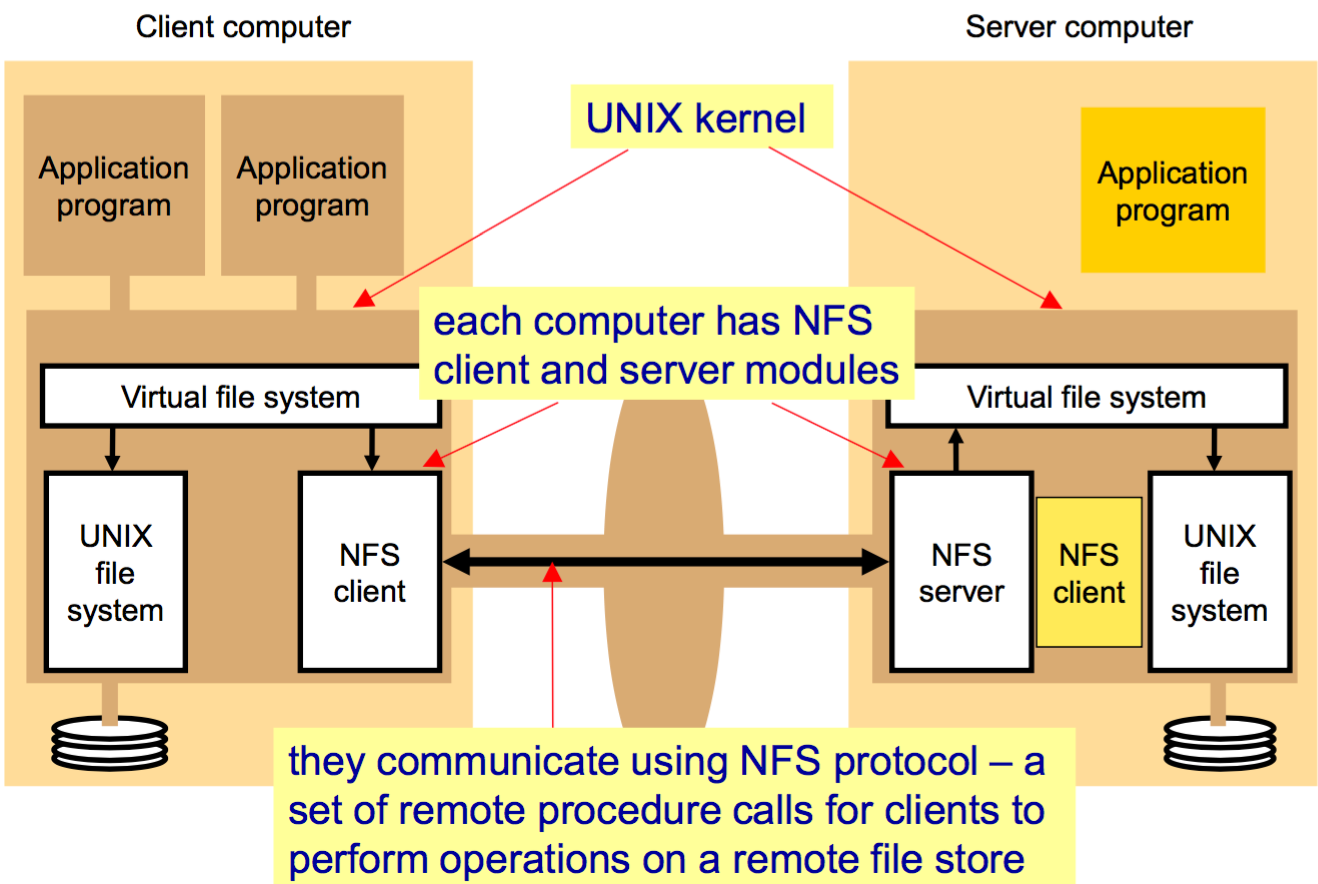
\includegraphics[width=8cm]{sun-file-system}
\end{center}

\noindent Each computer can act as both a client and a server.

\noindent File are accessed by file identifiers. File identifier is independent of the file name, created by the server hosting the file system and unique with respect to all files in the system. 

\section{Client-Server Communication}
\noindent NFS server operations are stateless and idempotent, so at-least-once invocation semantics can be used\\

\noindent NFS client operations need to supply an interface suitable for use by conventional application programs. The interface emulates UNIX file system semantics. \\

\noindent Mount service: file systems have to be exported by the server and be mounted by a client before they can be accessed by the client\\

Page 151 continue

Client Caching

Andrew and Coda File System

\end{multicols*}
